\documentclass{article}
\usepackage{url}
\usepackage{fullpage}
\usepackage[utf8]{inputenc}
\begin{document}
\title{Let's build electrostatic headphones}
\author{Arno Mayrhofer}
\maketitle

\tableofcontents

\newpage

\section{Introduction}
\label{s:intro}
The following document will describe the journey on how to construct your own electrostatic headphones starting with zero, zilch, nada, niente and nichts. In Section \ref{s:tools} we will list the tools required for the building process, which will be followed by a list of materials in Section \ref{s:materials}. The actual construction process is split into five parts, the building of the driver (Section \ref{s:driver}), enclosure (Section \ref{s:driver}), headband (Section \ref{s:headband}) and earpads (Section \ref{s:pads}) with a final assembly in Section \ref{s:assembly}. Finally, the last two chapters will deal with measurements (Section \ref{s:measurements}) and things that we would do differently for the second pair (Section \ref{s:future}).

The whole construction is based on the Head-Fi.org thread \cite{head-fi-diy-thread}, with different and more detailed sources (e.g. \cite{electrostatic-hp-design}, \cite{tcengineering-electrostatic-drivers}) given in the respective sections.

\begin{figure}[htb]
    \centering
    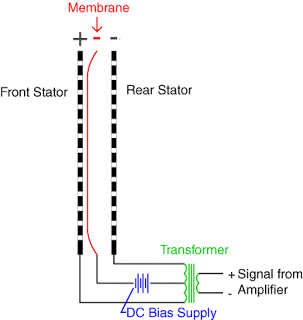
\includegraphics[width=0.5\textwidth]{images/esl_animation.png}
    \caption{Electrical concept}
    \label{f:intro:e-concept}
\end{figure}

The basic electrical concept of a electrostatic headphone can be seen in Fig. \ref{f:intro:e-concept}. An amplifier provides an input signal that is then transformed to yield the desired output voltage that drives the two stators. Additionally, there is a negative DC current that keeps the diaphragm charged.

\section{Required tools}
\label{s:tools}

\section{Required materials}
\label{s:materials}
\begin{enumerate}
    \item 1 mm PCB (for stators and dust protection spacers)
    \item 0.5 mm (or 0.6 mm) PCB (for spacers)
    \item 3 $\mu m$ Mylar (for diaphragm)
    \item 1-2 $\mu m$ Mylar (for dust protection, 1 $\mu m$ too thin maybe as very fragile) %AM-TODO
    \item \ldots (for coating the diaphragm) %AM-TODO
    \item Sheep skin leather (headband and pads)
    \item Wood (enclosure)
    \item Metal rods (headband)
    \item Foam (pads and headband)
\end{enumerate}

For the amplifier:
\begin{enumerate}
    \item TODO
\end{enumerate}

\section{Building the driver}
\label{s:driver}

\subsection{Design of the stators and spacers}
\label{s:driver:design}
Radius of the holes should not be larger than the distance from stator to spacer. The holes in the stator should not cover the whole stator. Instead there should be a perimeter that acts as an air damper and avoids resonance frequencies in the upper midrange or lower treble. The size of the diaphragm is quite important as low frequencies require a large diaphragm surface. The active area should have a diameter of about 80 mm. The ratio of spacer thickness to diaphragm width should not be larger than 1:120 to avoid contact between stator and diaphragm. Lowering the bias voltage can help with very large ratios.

In order to protect the diaphragm a dust and sweat protection needs to be used. This dust cover will be made from crumpled Mylar and will be located on the same side as the coating of diaphragm.

\url{file:///home/arnom-private/projects/headphones/guide/hp/My\%20DIY\%20electrostatic\%20headphones\%20-\%20Page\%2045.html#post_8897170} -> Design pictures of the Orpheus clones; apparently this design lacks some bass punch, maybe increase non-holed perimeter for improvements?

\subsection{Etching the stators}
\label{s:driver:etching}
Etching the PCB board ensures that electrical contacts are only where they absolutely need to be. Furthermore, having less copper surface will result in a reduced capacitance and they will be easier to drive because of that. Toner transfer can be used to define the areas that should not be etched. After etching the stators can be protected by spraying thin layers of Acrylic paint on the copper. This insulation avoids degradation of the copper surface and potential shorts when dust is present between the diaphragm and the stators.

\subsection{Tensioning the Mylar diaphragm}
\label{s:driver:tension}
Mylar with 3 $\mu m$ thickness is used to create the diaphragm. Thinner Mylar will cause a lack of bass, while thicker one will cause problem in treble and mids.
Different ways of tensioning the Mylar:
\begin{enumerate}
    \item With weights on the side
    \item Using a bicycle tire and inflating it
    \item Using tape to stretch it
\end{enumerate}
\begin{figure}[htb]
    \centering
    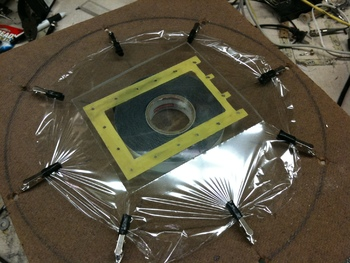
\includegraphics[width=0.5\textwidth]{images/mylar-tension-weight.png}
    \caption{A Mylar tensioning rig using weights}
    \label{f:driver:tension:weight}
\end{figure}
\url{http://www.head-fi.org/t/498292/my-diy-electrostatic-headphones/720#post_9217468} -> Orpheus clone tensioning

Before putting it on the glass (and before coating) clean it with Acetone. To cut the Mylar after glueing use a soldering iron.

After glueing the Mylar onto the spacers knock them on the side of a table to check that the sound of both diaphragms is similar. If not, a hot air gun can be used to tension the one with a looser sound.

\subsection{Coating the diaphragm}
As Mylar is not conductive an additional coating is required so that it can be charged. It basically should act as if it was a capacitor, so a coating that is conductive and has a high resistivity is ideal. Coating agents are:
\begin{enumerate}
    \item Staticide 6300 (anti static cleaner for monitors)
\end{enumerate}
Coating is achieved by applying a small drop of Staticide onto the diaphragm and then spreading it with a sponge.

Thread about coating: \url{http://www.diyaudio.com/forums/planars-exotics/109789-esl-diaphragm-coating.html}

Is this Staticide a gel?

\subsection{Assembly}
\label{s:driver:assembly}
Synthetic rubber glue (contact cement) is used to glue the diaphragm to the spacers. The dust protection screen must also be placed on some spacers (1mm thickness PCB) and must not be in contact with the stators. 2 $\mu m$ Mylar is crumpled and then stretched somewhat so that it doesn't touch the stators when on the spacer. This yields an ideal acoustically transparent material for dust protection. Normally, no dust cover is used on the outside. As no sweat protection is required on this side a very fine cloth could be used if needed. Only one spacer is glued to the diaphragm. This spacer will be the one facing the outside. The spacer on the inside will have the copper side in contact with the coated diaphragm and will be the one with the electrical contact to the DC bias voltage.
\begin{figure}[htb]
    \centering
    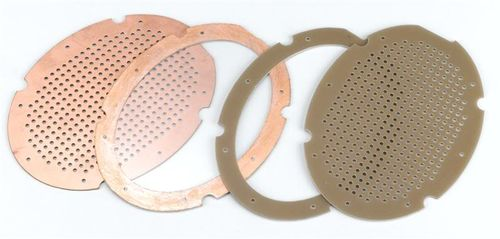
\includegraphics[width=0.5\textwidth]{images/arrangement.png}
    \caption{Arrangement and orientation of stators and spacers (missing the dust protection spacer and film)}
    \label{f:driver:assembly:arrangement}
\end{figure}

Plastic screws are used to assemble the driver unit.

The driver can be tested by hooking it up to the amp and leave it as is for 3 to 4 hours without playing any music. The diaphragm should not be sucked to one side during this.

\subsection{TODO}
\begin{enumerate}
    \item What does it mean to bias the headphone for a certain voltage?
    \item What is used to coat the diaphragm? Coating is done with a wet sponge maybe.
    \item How much does the Mylar need to be stretched ($< 1\%$)?
    \item How to do accurate etching and what chemicals should be used? FeCl or HCl are options
    \item How can the surface resistance of the diaphragm be measures? Simply measure at opposite sides? Check multimeter capabilities as it might not be able to measure resistance in the GOhm range. Try to find alternative ways of measuring resistance if that is the case.
\end{enumerate}

\subsection{Potential improvements}
\begin{enumerate}
    \item Drill holes with two different sizes to get a larger hole to surface area ratio
\end{enumerate}

\section{Building the enclosure}
\label{s:enclosure}
Wooden enclosures are potentially problematic as they can attract moisture which can cause electrical leakage. Sennheiser uses varnish on the outside of their wooden cups but none on the inside. It is possible to use a plastic O-ring to avoid direct contact between the wood and the driver.

\section{Building the headband}
\label{s:headband}

\url{file:///home/arnom-private/projects/headphones/guide/hp/My\%20DIY\%20electrostatic\%20headphones\%20-\%20Page\%2046.html#post_8943826}

\section{Building the earpads}
The earpads should be thick enough so that the bass is powerful and deep enough.
\label{s:pads}
\subsection{Potential improvements}
\begin{enumerate}
    \item Material should be leather on the inside. Sennheiser HE60/90 has fabric in contact with head, leather everywhere else. This makes it more comfortable
    \item It might be worth having harder foam on the inside as it will reduce resonances. Obviously this needs to be balanced to ensure comfort.
    \item Is it possible to make individual ear pads? Would allow for the use of harder materials. Moving your mouth changes the geometry so one would need to be careful.
\end{enumerate}
Post on ear pads: \url{file:///home/arnom-private/projects/headphones/guide/hp/My\%20DIY\%20electrostatic\%20headphones\%20-\%20Page\%2045.html#post_8930271}

\section{Assembly}
\label{s:assembly}
Cables should be doubly insulated to withstand the high voltage. DIN plugs are used by many for electrostatic headphones but it might not be safe due to the high voltages, same for XLR.

\subsection{TODO}
\begin{enumerate}
    \item Cable building (low capacitance)
    \item Connector building: need 6 pins ideally (3 for each side, for front and rear stator as well as one for the diaphragm DC voltage)
\end{enumerate}

\section{Amplifier}
\label{s:amp}
Due to the requirement of a continuously charged diaphragm and the high voltage requirements of the stators a dedicated amplifier is required for electrostatic headphones.
\begin{figure}[htb]
    \centering
    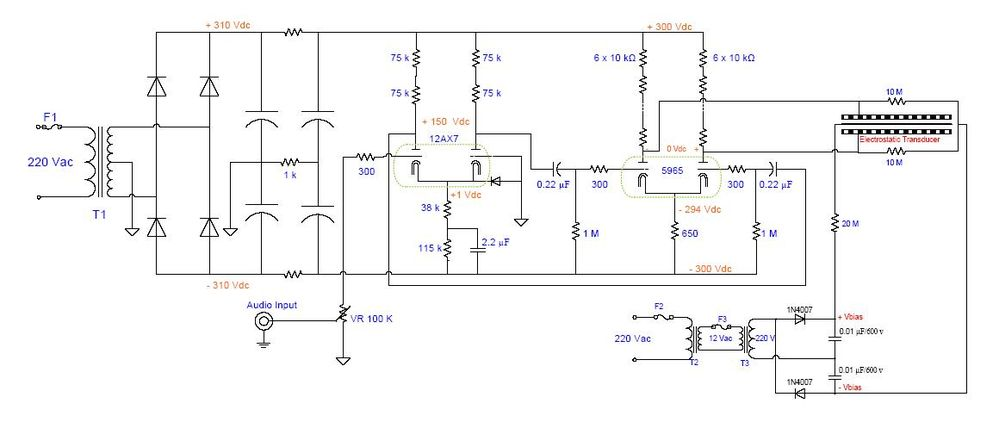
\includegraphics[width=0.5\textwidth]{images/wachara-amp.png}
    \caption{Amplifier design by Wachara C.}
    \label{f:amp:wachara}
\end{figure}
Discussion on this design: \url{file:///home/arnom-private/projects/headphones/guide/hp/My\%20DIY\%20electrostatic\%20headphones\%20-\%20Page\%2049.html#post_9182523}. Probably a step up transformer will be enough for starters

Other amplifier and transformer designs can be found here: \url{https://jazzman-esl-page.blogspot.co.at/2010/01/update-new-toroidal-step-up.html}

\section{Measurements}
\label{s:measurements}

Measurements with and without seal should be performed. The latter should give a peak at around 200 Hz which is the free-air resonance frequency. This frequency should be lower than 150 Hz for a good bass response.

\section{What to do different in the future}
\label{s:future}

\subsection{Closed headphones}
\label{s:future:closed}
Materials used for damping included felt, wool or other acoustically semi-transparent materials. Some also coat the inside of the enclosure with Bitumen.


\bibliographystyle{plain}
\bibliography{main}

\end{document}
